% Propósito: distinguir los tres componentes mínimos de una situación acústica.
% Origen: esquema conceptual fuente--medio--receptor de la Unidad 1.
% Descripción accesible: tres bloques, Fuente, Medio y Receptor, conectados en
% ese orden; la perturbación se origina en la fuente, se propaga por el medio y
% produce una respuesta en el receptor.
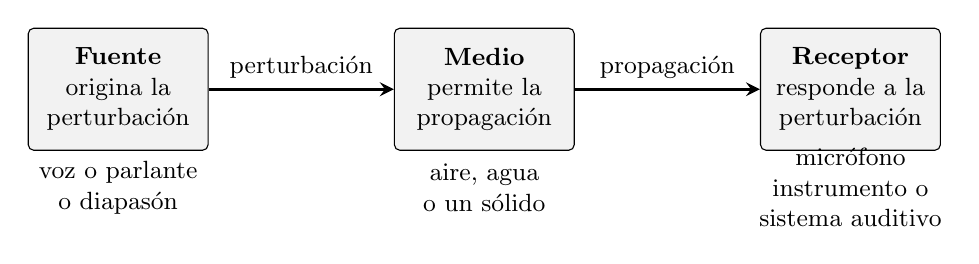
\begin{tikzpicture}[
    font=\small,
    >=stealth,
    bloque/.style={
        draw,
        rounded corners=2pt,
        text width=2.05cm,
        minimum height=1.55cm,
        align=center,
        fill=black!5
    }
]
    \node[bloque] (fuente) at (0,0)
        {\textbf{Fuente}\\origina la\\perturbación};
    \node[bloque] (medio) at (4.65,0)
        {\textbf{Medio}\\permite la\\propagación};
    \node[bloque] (receptor) at (9.3,0)
        {\textbf{Receptor}\\responde a la\\perturbación};

    \draw[->,very thick] (fuente.east) -- node[above]{perturbación} (medio.west);
    \draw[->,very thick] (medio.east) -- node[above]{propagación} (receptor.west);

    \node[align=center] at (0,-1.25) {voz o parlante\\o diapasón};
    \node[align=center] at (4.65,-1.25) {aire, agua\\o un sólido};
    \node[align=center] at (9.3,-1.25) {micrófono\\instrumento o\\sistema auditivo};
\end{tikzpicture}
